
\documentclass[a4paper]{article}
\usepackage[french]{babel}
\usepackage[utf8x]{inputenc}
\usepackage{xcolor}
\usepackage{graphicx}
\usepackage{amsmath}
\usepackage{lipsum} % Package to generate dummy text throughout this template
\usepackage{tikz}
\usepackage{enumerate}
\usepackage[sc]{mathpazo} % Use the Palatino font
\usepackage[T1]{fontenc} % Use 8-bit encoding that has 256 glyphs
\usepackage{setspace}
\onehalfspacing
\usepackage{microtype} % Slightly tweak font spacing for aesthetics

\usepackage[margin=4cm]{geometry} % Document margins
\usepackage[hang, small,labelfont=bf,up,textfont=it,up]{caption} % Custom captions under/above floats in tables or figures
\usepackage{booktabs} % Horizontal rules in tables
\usepackage{float} % Required for tables and figures in the multi-column environment - they need to be placed in specific locations with the [H] (e.g. \begin{table}[H])
\usepackage{hyperref} % For hyperlinks in the PDF

\usepackage{lettrine} % The lettrine is the first enlarged letter at the beginning of the text
\usepackage{paralist} % Used for the compactitem environment which makes bullet points with less space between them
\usepackage{multirow}
\usepackage{abstract} % Allows abstract customization
\renewcommand{\abstractnamefont}{\normalfont\bfseries} % Set the "Abstract" text to bold
\renewcommand{\abstracttextfont}{\normalfont\small\itshape} % Set the abstract itself to small italic text

\usepackage{titlesec} % Allows customization of titles
\renewcommand\thesection{\Roman{section}} % Roman numerals for the sections
\renewcommand\thesubsection{\arabic{subsection}} % Roman numerals for subsections
\titleformat{\section}[block]{\large\scshape\centering}{\thesection.}{1em}{} % Change the look of the section titles
\titleformat{\subsection}[block]{\large}{\thesubsection.}{1em}{} % Change the look of the section titles

\usepackage{fancyhdr} % Headers and footers
\pagestyle{fancy} % All pages have headers and footers
\fancyhead{} % Blank out the default header
\fancyhead[C]{Projet $\bullet$ Base de Données et Web $\bullet$ Stephan Morley Pegge $\bullet$ 2013-2014} % Custom header text


%----------------------------------------------------------------------------------------
%	TITLE SECTION
%----------------------------------------------------------------------------------------

\title{\vspace{-4mm}\rule{13cm}{0.2pt}\\[0.4cm]
\fontsize{18pt}{15pt}\selectfont\textbf{Base de Données et Web}\\[0.1cm]
\fontsize{11pt}{10pt}\selectfont{Géolocalisation de stations de Vélib' et de musées à Paris}\\[0.4cm]
\rule{13cm}{1.4pt}} % Article title
\date{}




\begin{document}

   \begin{flushright}
   \textsc{Edouard DAOU -- Clement DELL'AEIRA \\
     Cuong NGUYEN QUOC -- Florent RITLENG}\\
   ENSAE ParisTech \\
   2013-2014\\
   \vspace{-5mm}
   \end{flushright}
   \begingroup
   \let\newpage\relax% Void the actions of \newpage
\maketitle
\endgroup



\section{Introduction}
Dans le cadre de notre projet nous avons créé un site qui repose sur l'utilisation de bases de données SQL. L'interface du site est construite grâce aux langages PHP, CSS et Javascript. Nous utilisons plusieurs outils classiques comme des formulaires, des boutons checkbox\dots. 
\paragraph{Objectif du site}Notre site permet aux utilisateurs de repérer sur une carte des stations Vélib' et musées dans une zone de leur choix. Le site donne aussi la possibilité de s'enregistrer afin de sauvegarder des stations favorites ou des musées favoris.    
 
\section{Description des bases}

L'objet de cette partie consiste à présenter les bases de données que nous avons utilisées dans le cadre du projet. 

\subsection{Base Vélib' : \textbf{velib}}

La première base que nous avons utilisée provient du site data.gouv.fr et répertorie l'ensemble des 1230 stations de Vélib' présentes à Paris et dans sa région. La base de données comprend pour chaque station le numéro, le nom, l'adresse, le code postal, la ville et les coordonnées géographiques (latitude et longitude). La clef primaire de cette base est le champ "number".

\subsection{Base Monuments : \textbf{musee}}

La seconde base de données que nous avons utilisé provient également du site data.gouv.fr et répertorie 140 musées présents en Île-de-France. La base de données fournit pour chaque musée le nom, l'adresse, le code postal, la ville et les coordonnées géographiques. La clef primaire est le champ "id\_musee".

\subsection{Base d'utilisateurs : \textbf{members}}

Chaque utilisateur du site peut s'enregistrer afin de sauvegarder ses stations de Vélib' favorites et ses musées préférés. Pour ce faire, une base de données \textbf{members} est créée afin de mémoriser le pseudo, le mot de passe, l'adresse email, la clef de cryptage. Le mot de passe est crypté via l'algorithme \href{http://pajhome.org.uk/crypt/md5/sha512.html}{hashing algorithm sha512}. La clef primaire est le champ "id\_user" qui s'auto-incrémente lors de l'enregistrement d'un nouvel utilisateur. 

\subsection{Bases des favoris : \textbf{velib\_favorite} et \textbf{musee\_favorite}}

Une fois que l'utilisateur est enregistré, il peut s'il le souhaite répertorier ses stations de Vélib' et/ou ses musées favoris. Deux bases de données sont créees afin de stocker les préférences de chaque utilisateurs pour les stations de Vélib' (\textbf{velib\_favorite}) et les musées (\textbf{musee\_favorite}). Les clefs primaires associées à ces bases sont (id\_user,id\_velib) et (id\_user,id\_musee).


\section{Architecture du site}
Le site est constitué de 4 pages principales: 
\begin{itemize}
\item la page de recherche par code postal (\textbf{velib.php}) permet de rechercher les stations de Velib' et les musées franciliens par code postal.
\item la page de visualisation de stations Vélib'(\textbf{voir\_carte.php}) permet d'afficher sur une carte les stations de Vélib'. La recherche des stations voisines ou des musées alentours est également possible.  Si l'utilisateur est connecté, il peut ajouter une station dans ses favoris ou bien enlever une station de ses favoris. 
\item la page de musées (\textbf{voir\_musee.php})  permet de faire la même chose, mais pour les musées.  
\item la page de l'espace personnel (\textbf{connexion.php}) où un utilisateur peut se connecter ou bien s'enregistrer pour une première fois. La liste des favoris d'un utilisateur connecté sur le site est affiché sur cette page. 
\end{itemize}

Les trois dernières pages sont connectées entre elles : si un utilisateur clique sur une de ses stations favorites sur sa page personnelle, il sera redirigé sur la page de recherche de station vélib' et pourra continuer les requêtes sur celle-ci.\\

\begin{figure}[!h]\centering
\begin{tikzpicture}
\node[draw,thick,minimum width=2cm,minimum height=1cm,fill=gray!50] (rect) (A)at(2,4) {velib.php};
\node[draw,thick,minimum width=2cm,minimum height=1cm,fill=gray!50] (rect) (B)at(0,2) {voir\_carte.php};
\node[draw,thick,minimum width=2cm,minimum height=1cm,fill=gray!50] (rect) (C)at(4,2) {voir\_musee.php};
\node[draw,thick,minimum width=2cm,minimum height=1cm,fill=gray!50] (rect) (D)at(2,0) {connexion.php};

\tikzstyle{radial}=[very thick,->,>=stealth];
\draw[->,>=latex](A)--(C)
	node[midway,below]{};
\draw[->] (A)--(B)
	node[pos=0.1,above]{};
\draw[->] (A)--(C)
	node[pos=0.1,above]{};
\draw[->] (B)--(C)
	node[pos=0.1,above]{};  
\draw[->] (C)--(B)
	node[pos=0.1,above]{};    
\draw[->] (D)--(B)
	node[pos=0.1,above]{};
\draw[->] (D)--(C)
	node[pos=0.1,above]{};  
\end{tikzpicture}
\label{Archi}
\caption{Architecture du site}
\end{figure}

% Le mec qui a ecrit ça etait il bourré ?
%Le fonctionnement des pages de recherche repose sur des listes à choix multiples (pour le puis sur de la saisie de texte (pour le rayon) et enfin sur des checkbox afin de saisir les points d'intérêts qu'on aimerai voir sur la carte. 
%Plusieurs liens apparaissent donc entre les bases de données présentés dans la partie précédente. En effet \\
% partie reecrite (?)
Le fonctionnement des pages de recherche repose sur des listes à choix multiples et sur des checkbox. Un utilisateur entre par exemple son code postal, et choisit une station Vélib' dans la liste déroulante. Il peut alors, en choisissant la distance maximale qu'il veut parcourir, avoir accès à tous les musées qui se trouvent dans un disque de centre la station et de rayon la distance maximale. S'il clique sur le nom du musée, il bascule sur la page \textbf{voir\_musee.php}, et peut lire les informations enregistrées sur le musée. 

\clearpage
\section{Description du site}
\subsection{Page d'accueil}
\begin{figure}[!h]
\centering
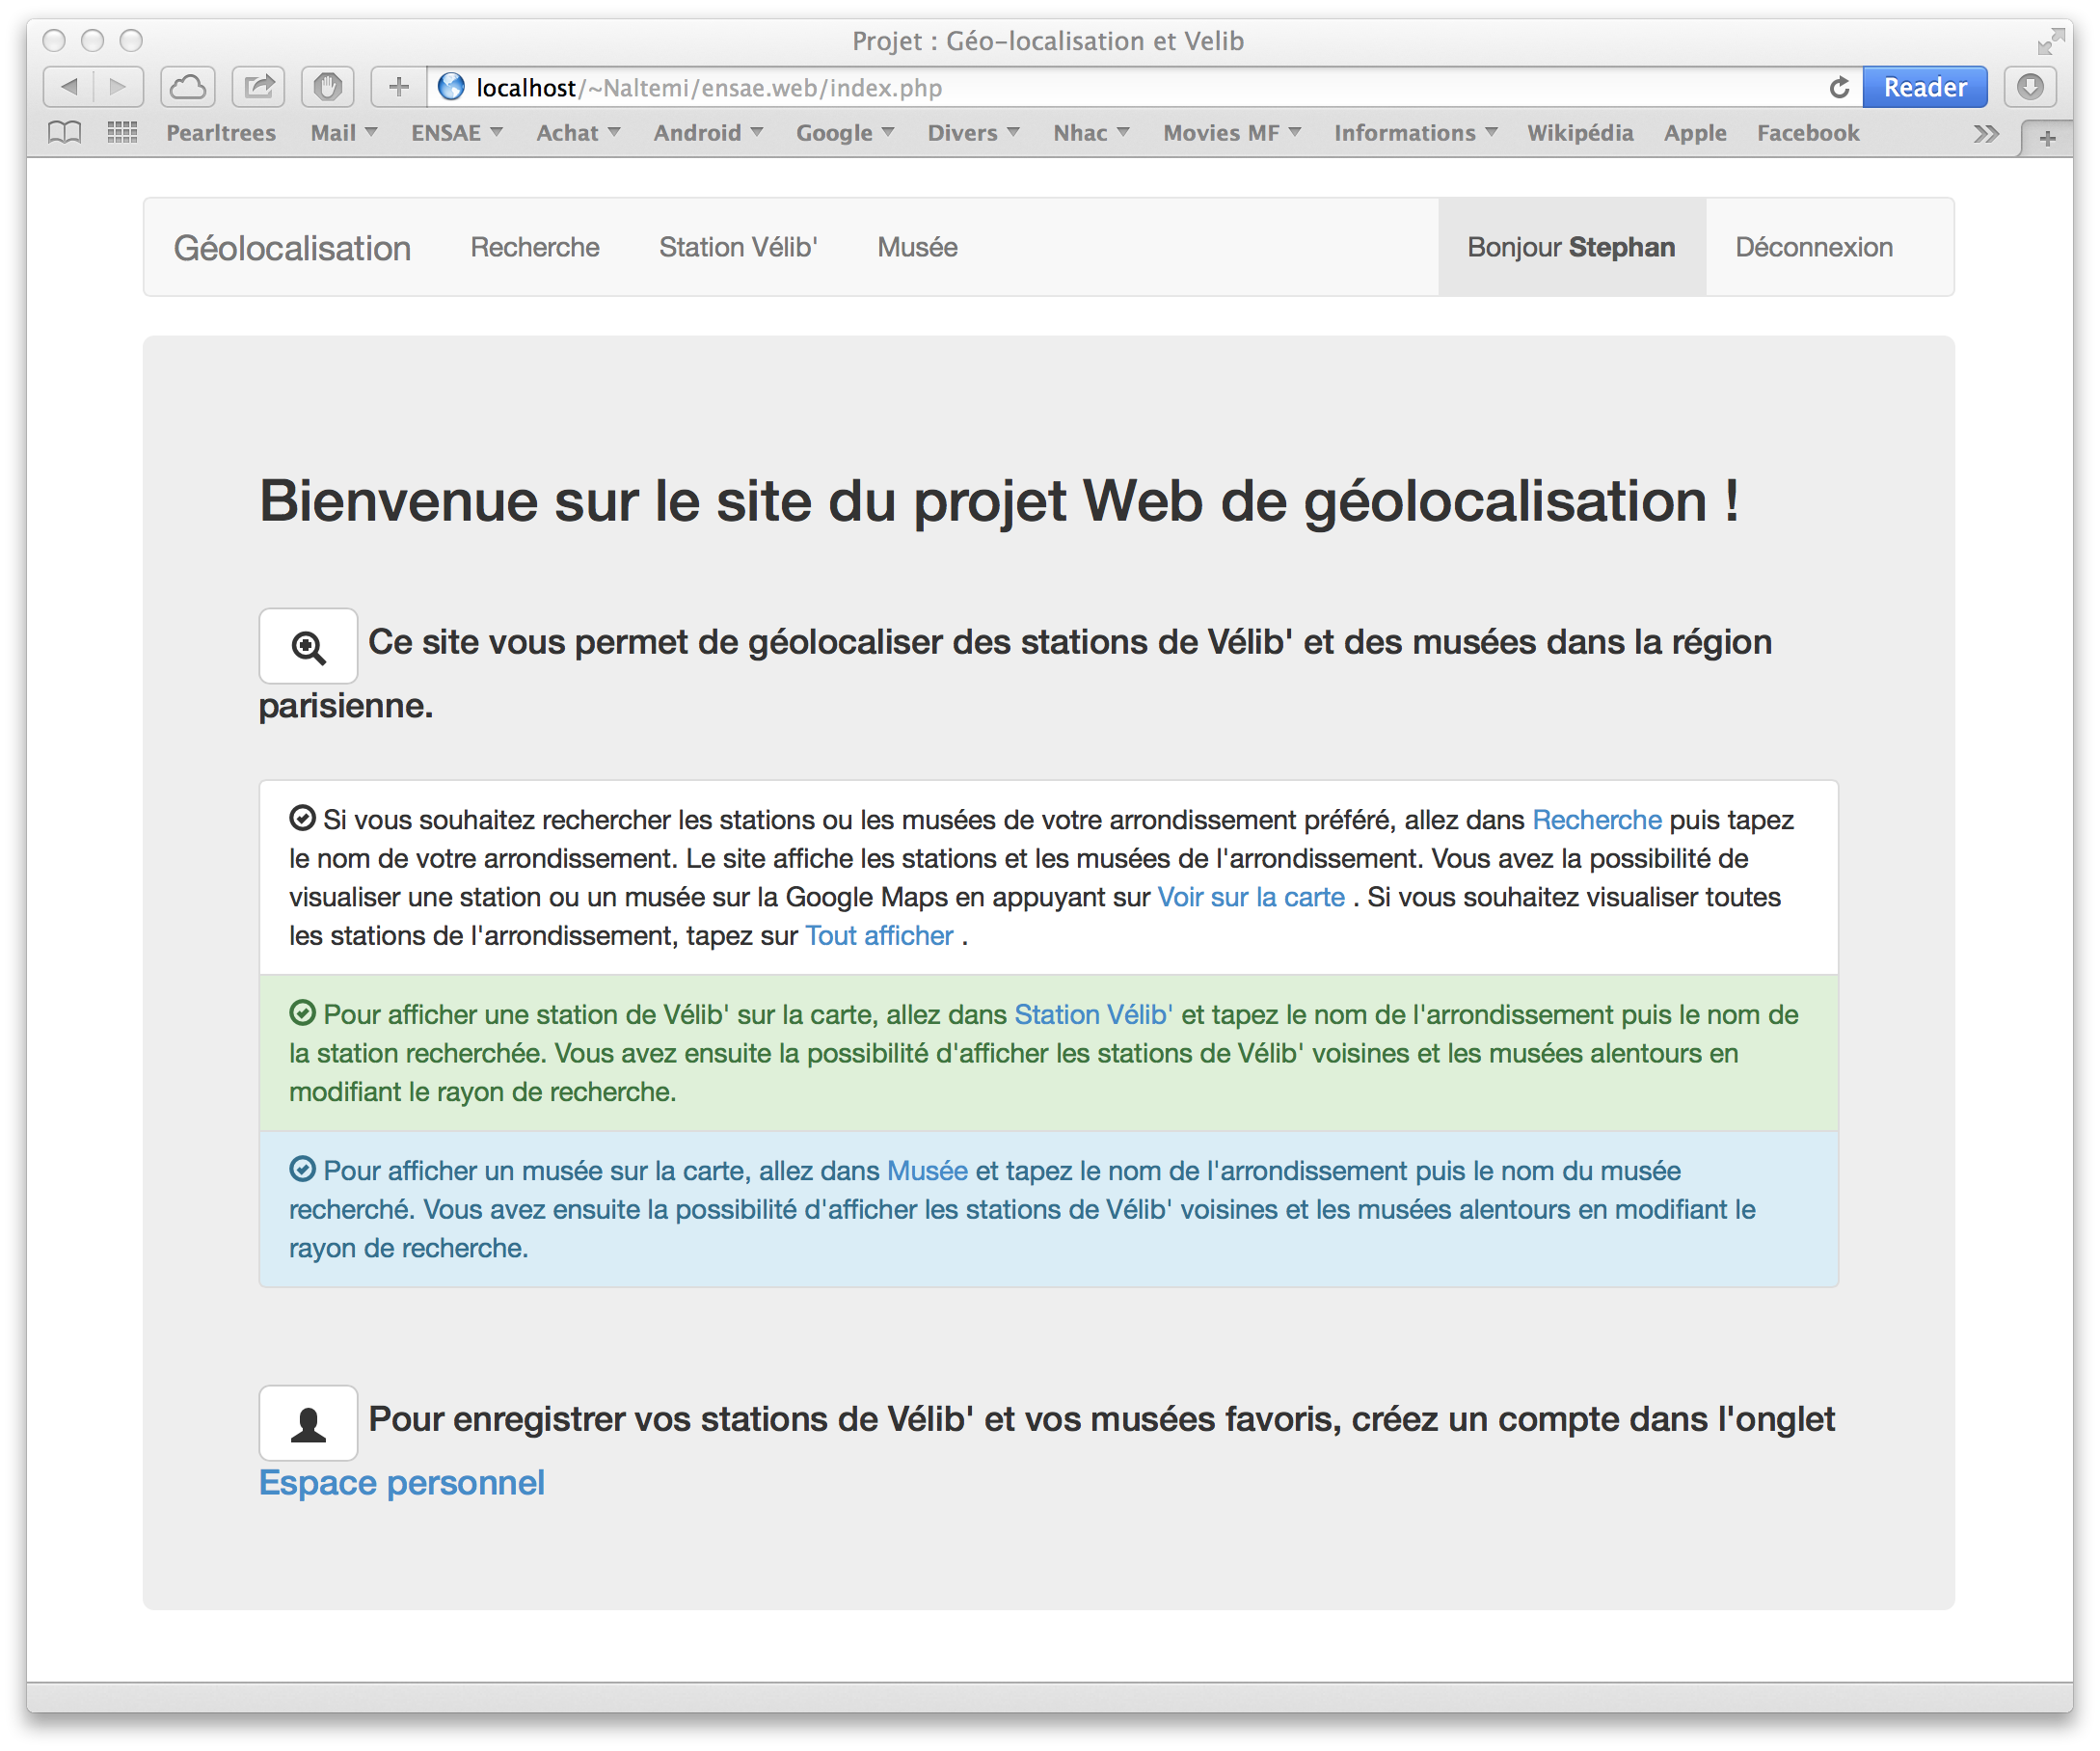
\includegraphics[scale=0.3,keepaspectratio=TRUE]{index}
\caption{Page d'accueil du site}
\end{figure}

\subsection{Visualiser les stations de Vélib'}
\begin{figure}[!h]
\centering

\includegraphics[scale=0.3,keepaspectratio=TRUE]{velib}
\caption{Page de visualisation des stations de Vélib'}
\end{figure}

\subsection{Espace Personnel}
\begin{figure}[!h]
\centering
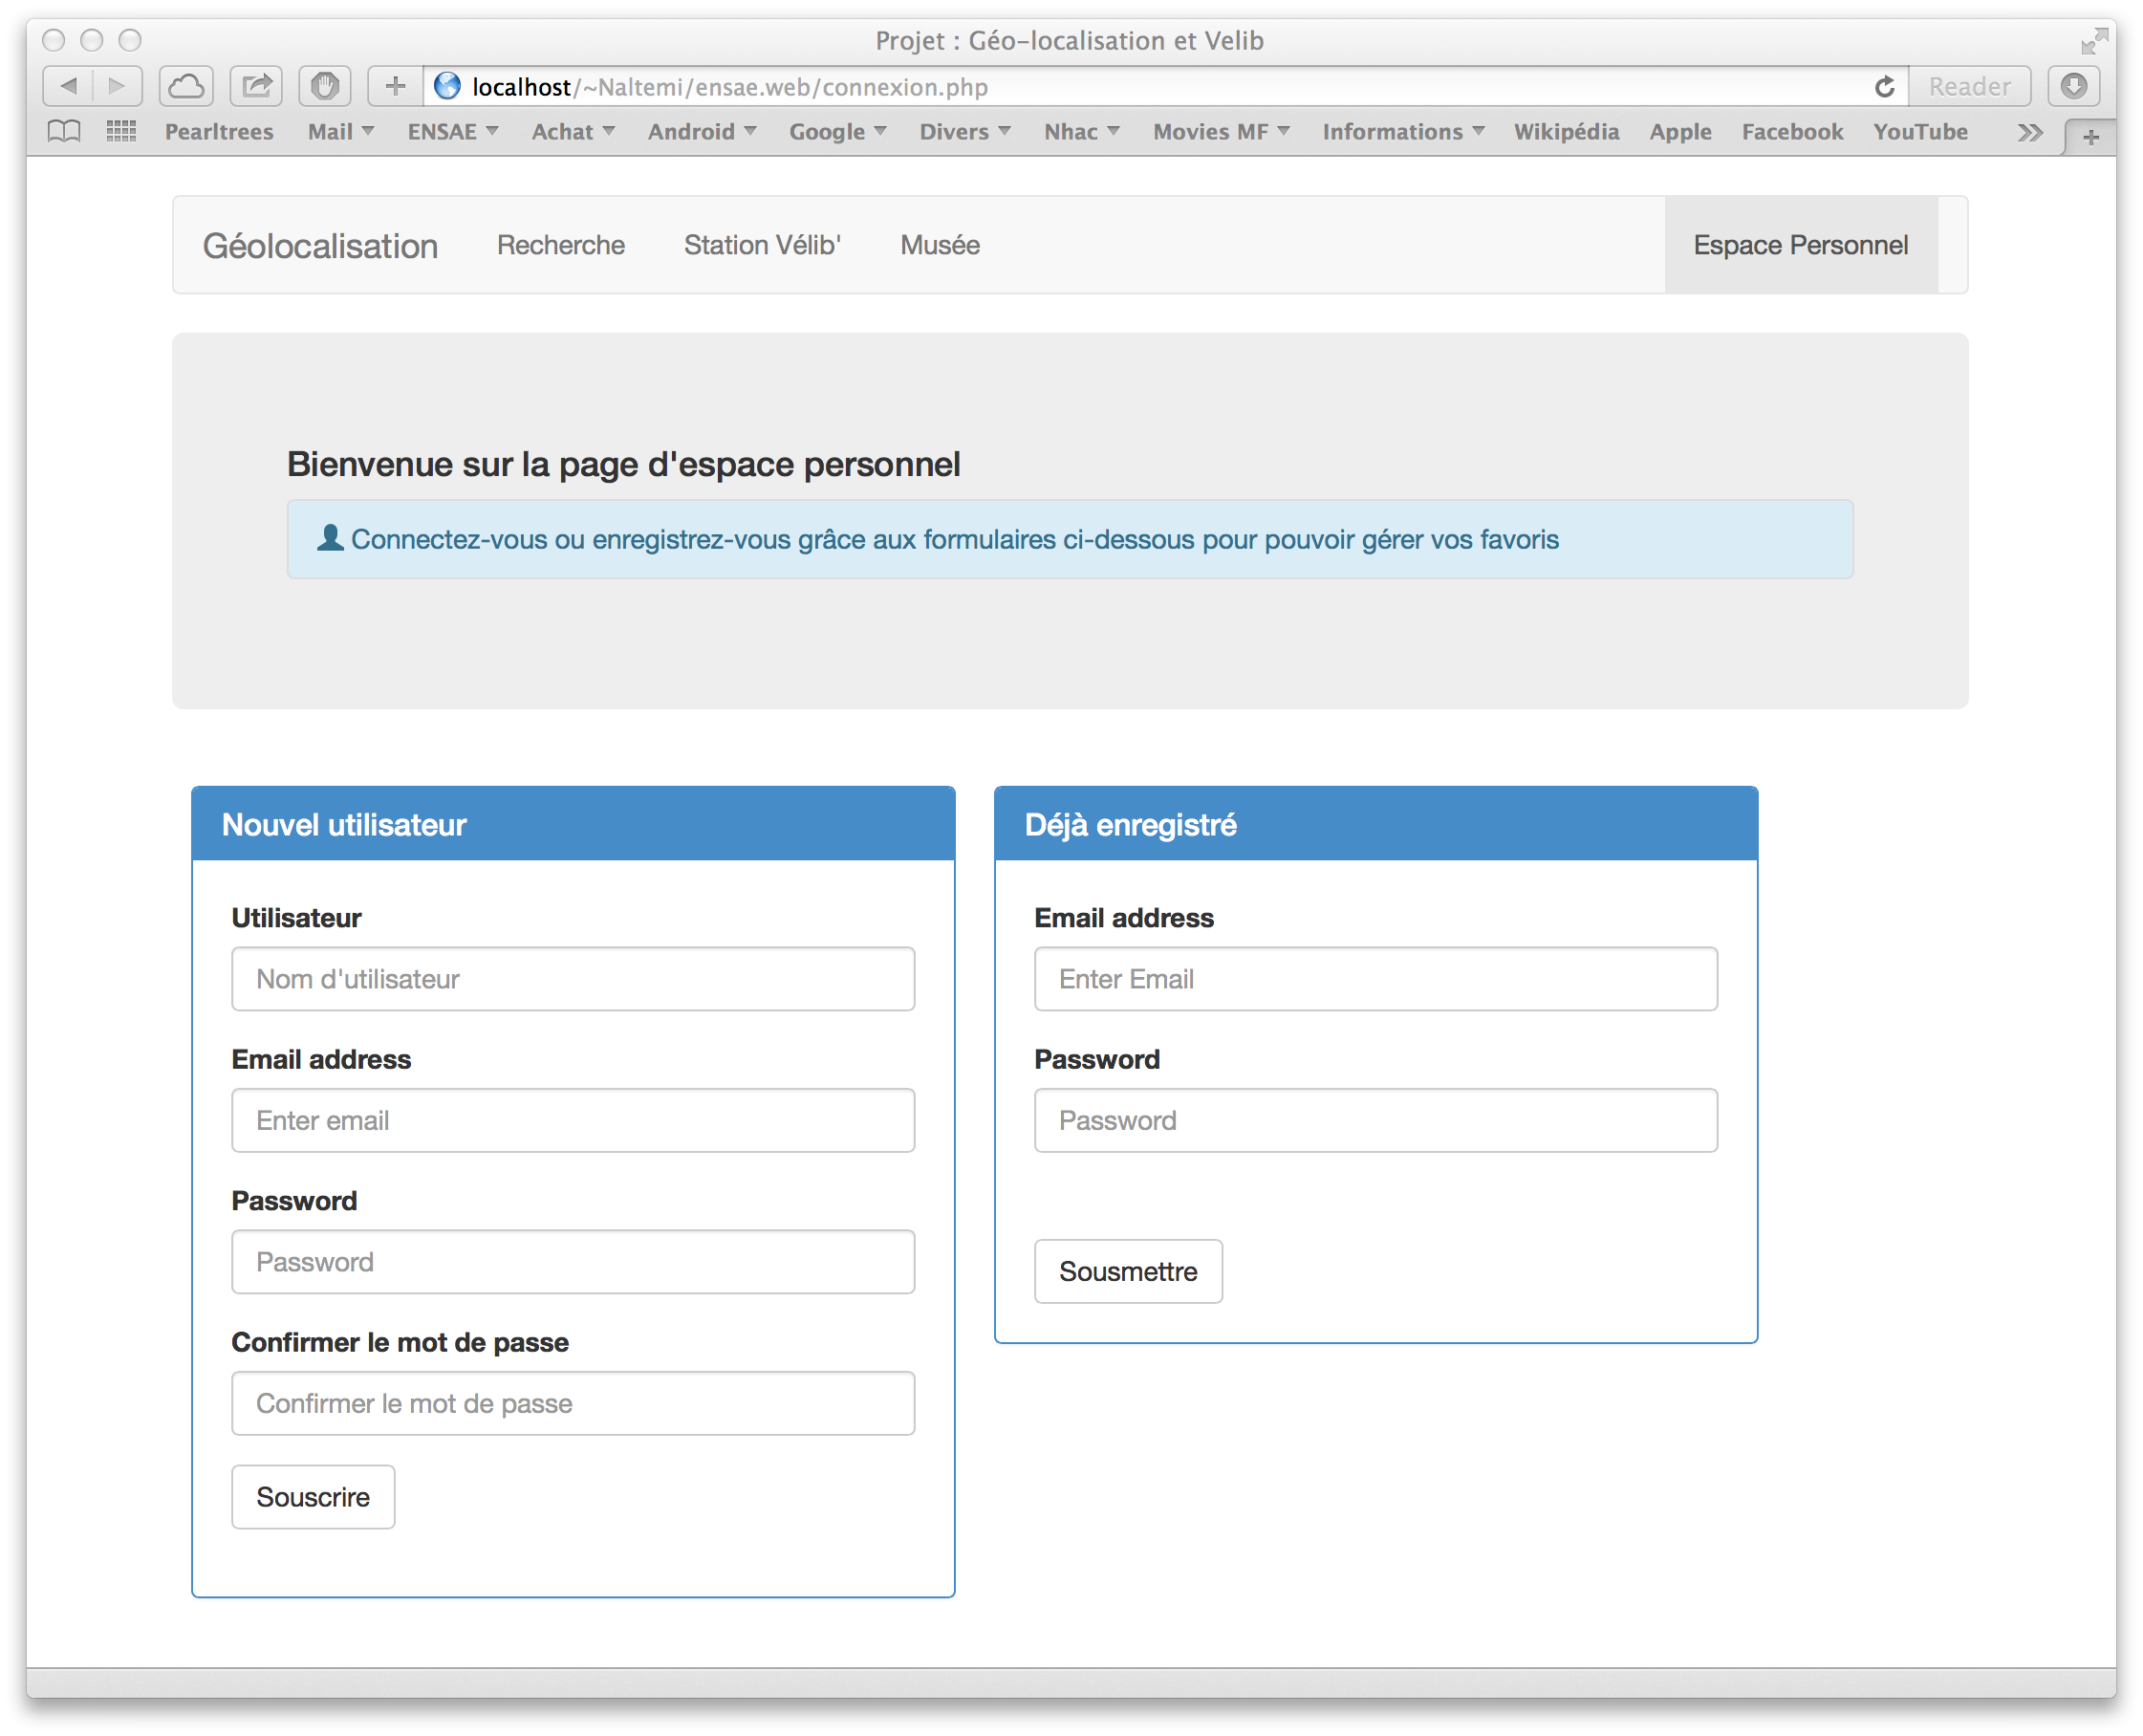
\includegraphics[scale=0.3,keepaspectratio=TRUE]{connexion_2}
\caption{Espace Personnel : Formulaire d'enregistrement et de connexion}
\end{figure}
\begin{figure}[!h]
\centering
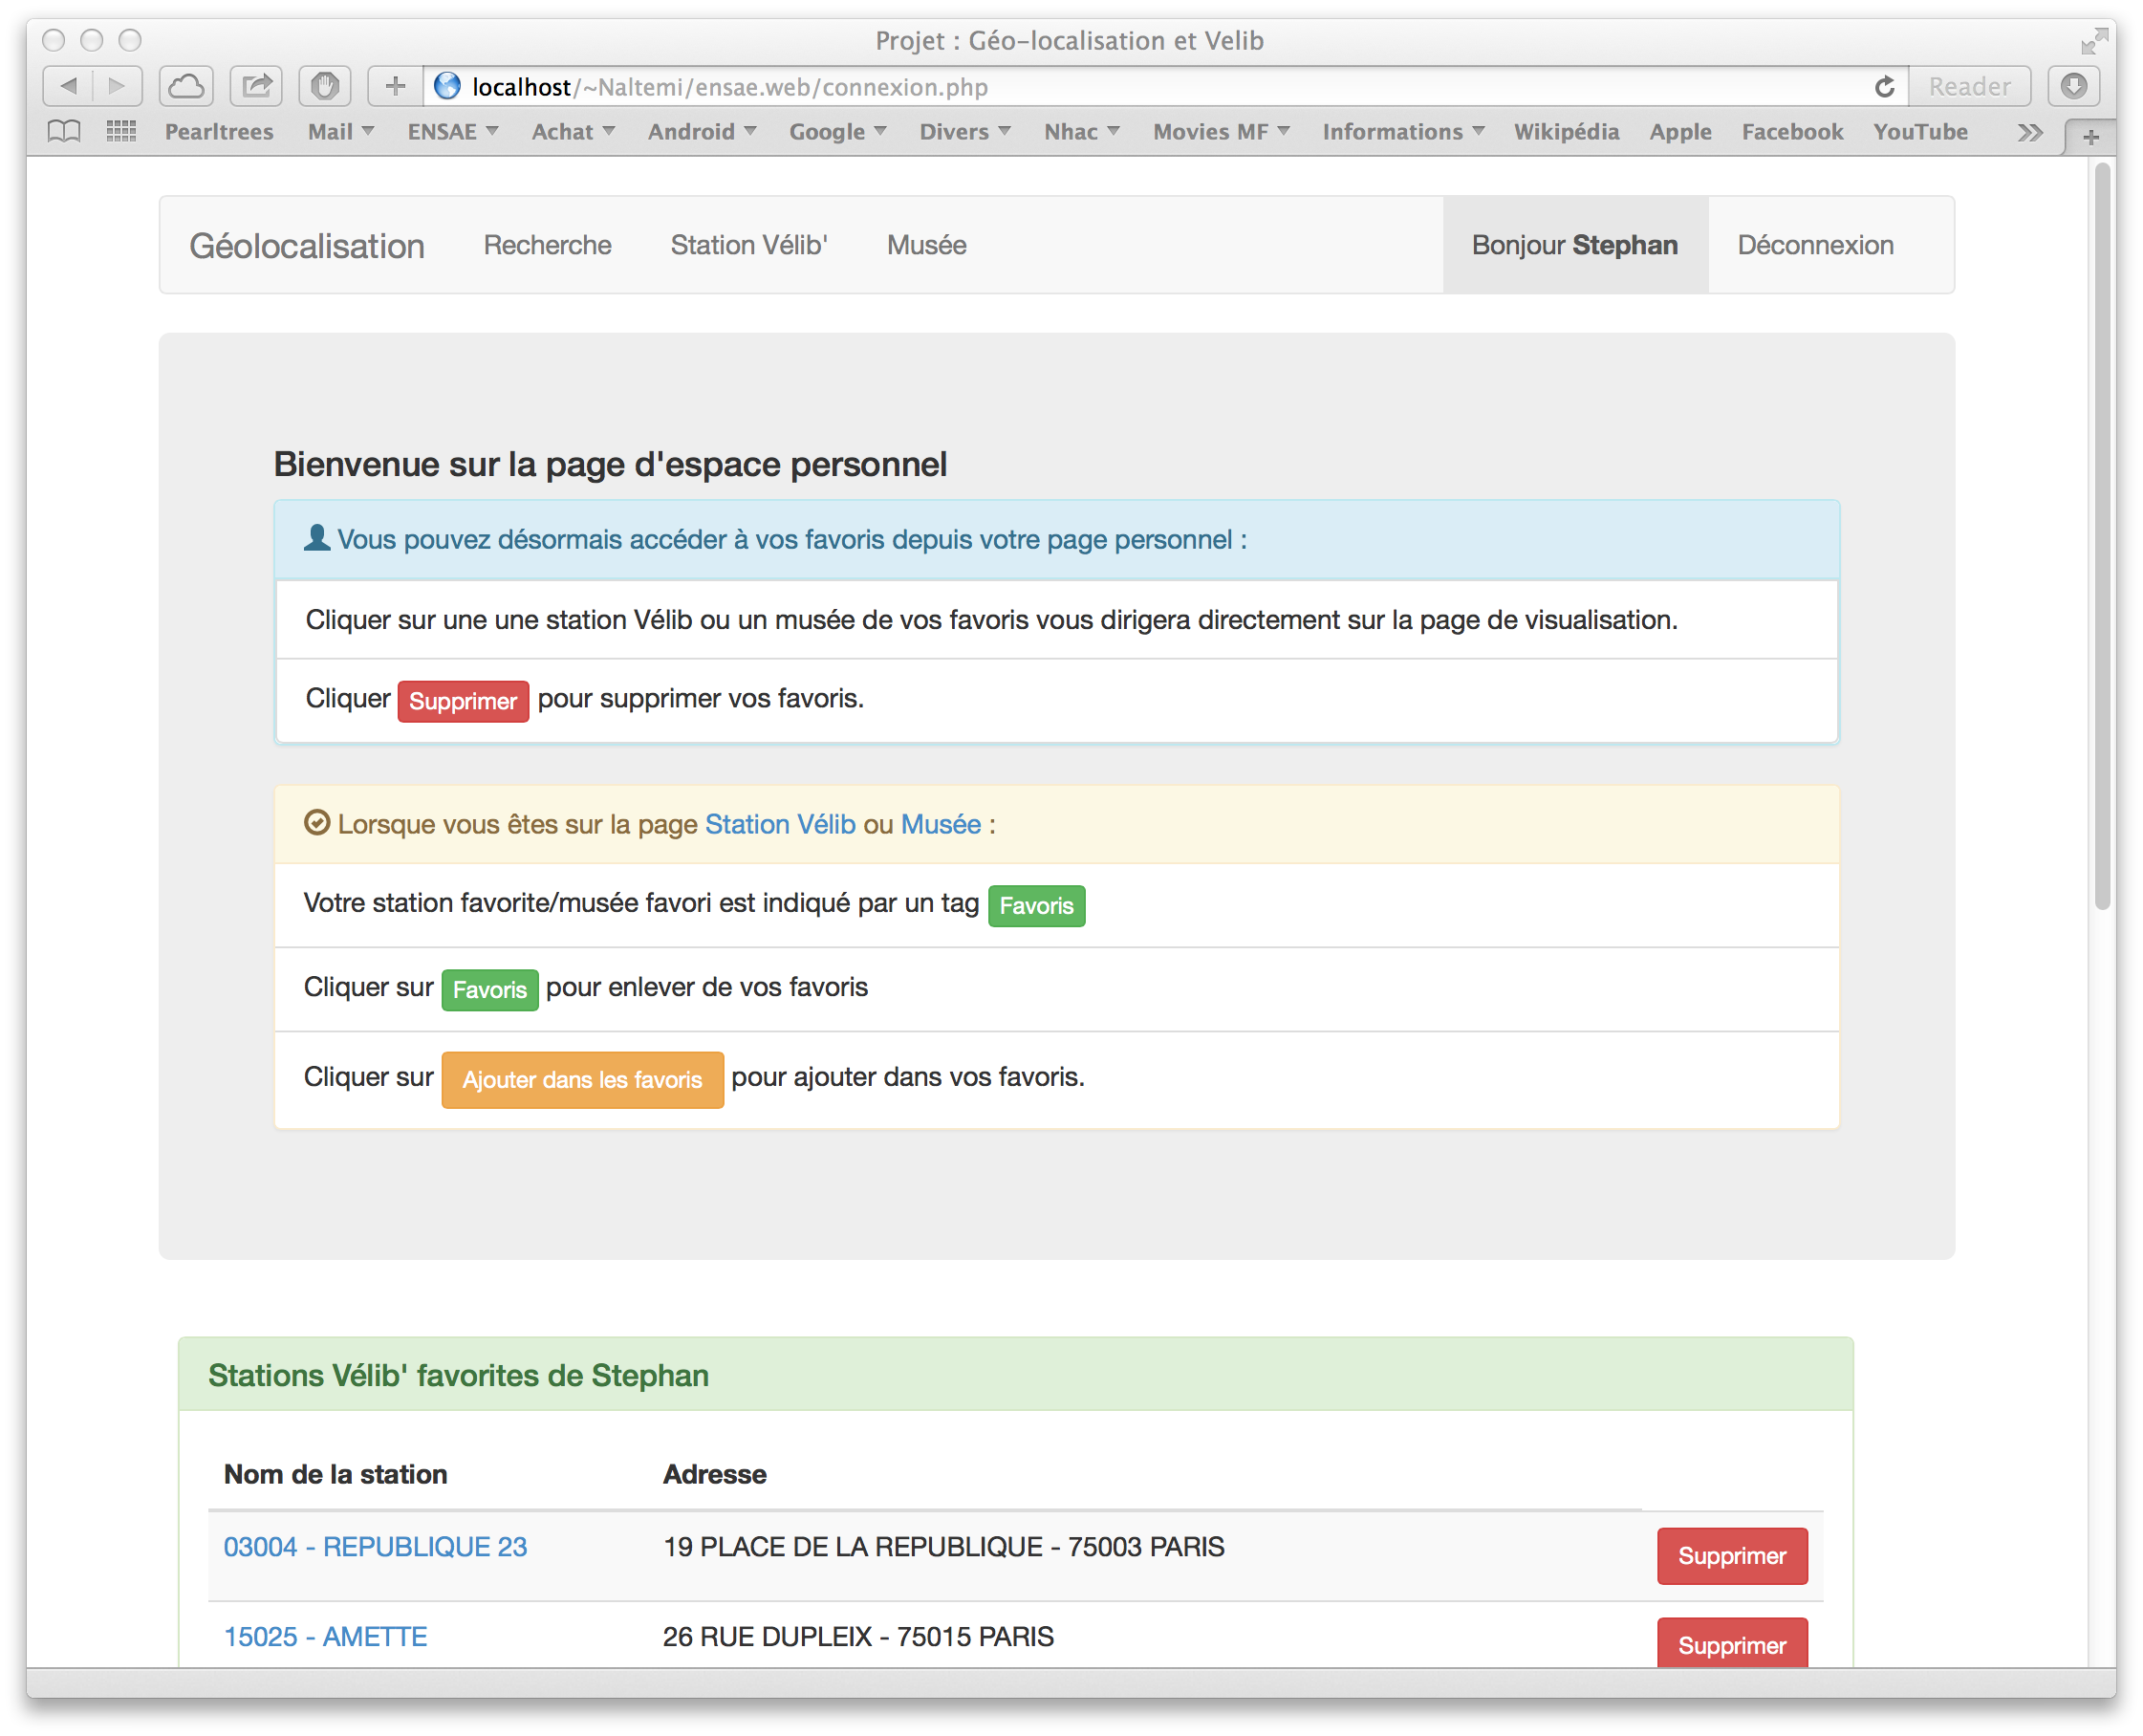
\includegraphics[scale=0.3,keepaspectratio=TRUE]{connexion_1}
\caption{Espace Personnel : Tableaux des points favorites}
\end{figure}

\end{document}